\subsection{Study Evaluation} \label{subsec:evaluation}

% Checking Cancer-Associated Genes
\subsubsection*{Evaluation of the Network with cancer-associated Genes} \label{subsubsec:evaluation_known_genes}
To evaluate the robustness of our network construction and PageRank algorithm,
we assess the placement of genes known to be involved in cancer development within our network.
Specifically, we examined a set of 9 genes identified as being associated with lung cancer
in a study by El-Telbany et al.~\cite{ElTelbany2012LungCancerGenes}.
We sought to determine whether these cancer-associated genes would emerge as hub nodes or exhibit high PageRank scores,
and how their expression levels $\Delta_{TPM}$ compare to those of other genes within our network.

We found that all 9 genes are present in our network,
which is a positive validation of the comprehensive coverage of our dataset.
Notably, the gene LKB1 is listed under the name STK11 in our data, which is a common alias for this gene.
\cref{fig:05_01_df_known_genes} provides an illustration of these genes
and their respective $\Delta_{TPM}$ values and PageRank scores.

\begin{figure}[!h]
    \centering
    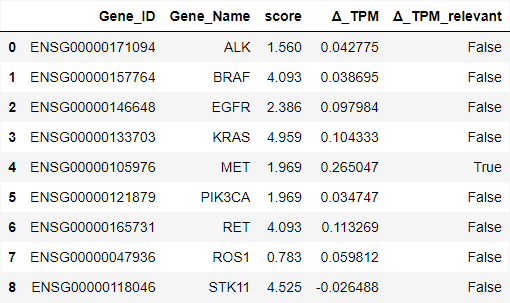
\includegraphics[height=\dfheightdouble]{figures/05_01_df_known_genes}
    \caption{9 known cancer-associated genes and their respective $\Delta_{TPM}$ values and PageRank scores}
    \label{fig:05_01_df_known_genes}
\end{figure}

When examining the placement of these cancer-associated genes within the network,
we observed that only one gene (with a $\Delta_{TPM}$ value of 0.265) is classified as $\Delta_{TPM relevant}$.
None of the others have a notable $\Delta_{TPM}$ value,
with most being situated in the middle of the distribution and showing no clear pattern or outliers.

Upon examining the placement of these cancer-associated genes, we observed that none of them have a PageRank score greater than 5,
which seems to be far away from the top 10 genes.
However, as shown in \cref{fig:05_known_genes},
4 of the 9 genes are situated within the top 10 percent of the distribution (PageRank score $>$ 3.67),
and all are above the median, indicating that they are relatively well-connected nodes within our network.

\begin{figure}[h]
    \minipage{0.45\textwidth}
        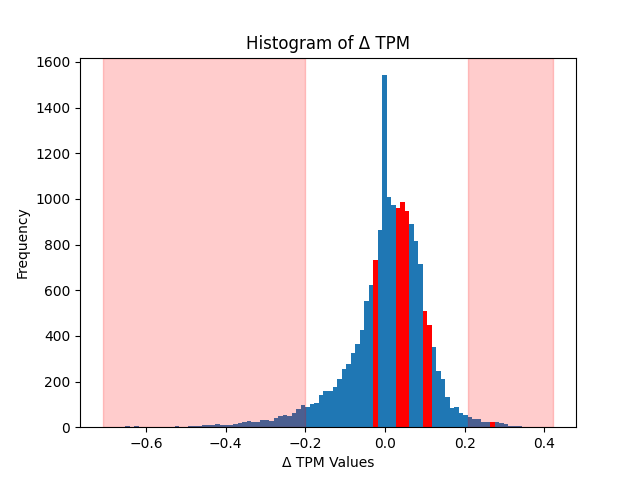
\includegraphics[width=\linewidth]{figures/05_01_delta_tpm_relevant}
    \endminipage
    \hfill
    \minipage{0.45\textwidth}
      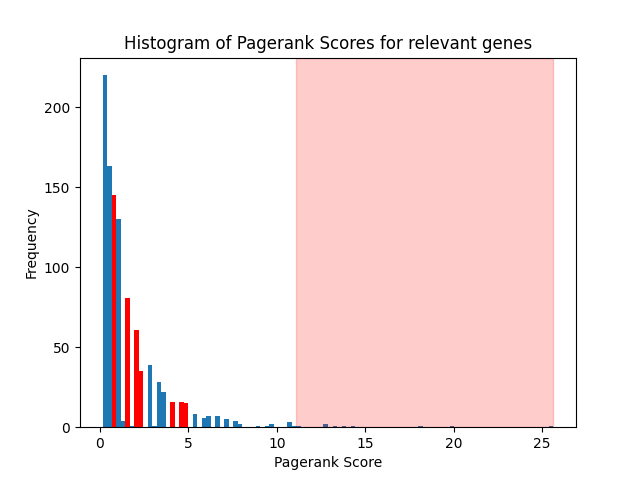
\includegraphics[width=\linewidth]{figures/05_01_pagerank_known_genes}
    \endminipage
    \caption{Distribution of the PageRank score and the $\Delta_{TPM}$
        with the area for significant change in gene activity highlighted in light red
        and the values for 9 known cancer-associated genes marked as red bars}
    \label{fig:05_known_genes}
\end{figure}

Our analysis suggests that while our network construction and PageRank algorithm are robust,
the placement of these cancer-associated genes within the network may not be directly indicative
of their role in cancer development.\\

%%%%%%%%%%%%%%%%%%%%%%%%%%%%%%%%%%%%%%%%%%%%%%%%%%%%%%%%%%%%%%%%%%%%%%%%%%%%%%%%%%%%%%%%%%%%%%%%%%%%%%%%%
% Delta TPM relevant
\subsubsection*{Limitation of the $\Delta_{TPM}$ and the $\Delta_{TPM relevant}$ measure} \label{subsubsec:limit_delta_tpm}
The calculated $\Delta_{TPM}$ values represent the relative difference in gene expression between normalized mean cancerous and healthy states,
indicating an increase or decrease in transcript abundance in the tumor compared to normal tissue.
We classified the significant 5\% of the genes as $\Delta_{TPM relevant}$ in our study.

The top 10 genes that we looked at all had a connection to cancer based on previous studies
- even if not all of them had a connection to lung cancer.
However, 10 genes is a rather small group to make a general statement of the quality of the delta TPM measure we developed.
By looking at the genes known for lung cancer, only one was classified as having relevant changes in gene activity.
This raises questions about the robustness and sensitivity of our approach.
While it seems like a solid starting point, there are some limitations and improvements that could be made based on the assumptions we made.

% what can be criticized? And how can it be improved?
One potential problem may be that our calculation assumes a linear relationship between healthy and cancerous TPM values
by subtracting the log-scaled mean TPM values.
Additionally, the log-scaled normalization method of TPM values might not be optimal,
and could be improved by using a different, e.g. non-linear method such as quantile normalization.
Furthermore, our measure may be too general, potentially leading to false negatives for genes that are more sensitive to smaller changes.
To address these concerns, it could be a way to investigate the correlation between cancerous and healthy tissues
with methods like fold change and enrichment scores.
Another improvement could be to use an additional measure such as FPKM or RPKM to validate the TPM results and not rely on only one measure.
\\

%%%%%%%%%%%%%%%%%%%%%%%%%%%%%%%%%%%%%%%%%%%%%%%%%%%%%%%%%%%%%%%%%%%%%%%%%%%%%%%%%%%%%%%%%%%%%%%%%%%%%%%%%
% PageRank
\subsubsection*{Limitation of the PageRank score} \label{subsubsec:limit_pagerank}
% How did it work?
PageRank is a well-established algorithm for ranking nodes in a network based on their connectivity.
Our assumption was that genes with more connections to other genes over their proteins would have a higher PageRank score,
meaning that their change in gene activity has a higher influential within the network.
Therefore we calculated the PageRank score for each gene in our network to determine its importance within the network
and find the most influential genes based on their connections.


% Did it work well?
However, upon examining the distribution of PageRank scores, we observed a trend with a few genes having high scores
and most genes having low scores.
This distribution suggests that a small number of highly connected nodes dominate the network's topology.

Our analysis revealed some interesting insights into how the PageRank score is distributed in our setup.
It appears that the score for a gene is largely influenced by the number of proteins it transcribes,
which corresponds to the number of first-level edges from the gene in the network.

This might be due to the relatively constant number of second-level edges (interactions between proteins),
making the PageRank score less informative than expected.

To address this issue, we propose exploring alternative approaches that consider multiple levels of interactions
or incorporate weights into the edges and nodes.

% inital Data
\subsubsection*{Limitation of the used datasets} \label{subsubsec:limit_base_data}

The quality and limitations of the datasets used in this study are critical factors that impact the validity and generalizability of our results.
While both the CMP and GTEx datasets provide valuable insights into gene expression and regulation,
they have some inherent limitations.

One notable aspect is that both datasets contain a large number of samples,
which could facilitate generalization to other populations.
However, it's essential to acknowledge that the age range of the participants in these studies might be biased towards older individuals.
As a result, our findings may not be representative of younger populations.
Since we were unable to find any information on ethnic diversity among the study participants for either the CMP or GTEx datasets,
it is unclear whether the results can be generalized to diverse populations.

Additionally, we have concerns about the accuracy of the matching of Ensemble ID names in the CMP dataset,
which could lead to incorrect gene assignments if not properly validated.
To address these limitations and improve the generalizability of our findings,
it could be an option to use alternative datasets such as TCGA, which is a widely used resource for cancer research.

Furthermore, it would be beneficial to incorporate datasets with diverse age ranges
and ethnic backgrounds to enhance the representativeness of our results.


% Conclusion
Our study provides a comprehensive analysis of the network of genes involved in lung cancer development.
Nevertheless, there are several limitations that should be addressed in future research.
One could be to investigate the correlation between the $\Delta_{TPM}$ and other measures such as fold change or enrichment scores
another could be to use additional datasets to validate the results and improve the generalizability of our findings.\\